El texto extraído de las redes sociales presenta desafíos y problemas específicos debido a la naturaleza única de estos datos. Algunos de los problemas comunes son:

\begin{itemize}

	\item Ruido y calidad del texto: Los datos de redes sociales suelen contener errores ortográficos, abreviaturas desenfrenadas, emojis, jerga, sarcasmo, uso  de mayúsculas inconsistentes, repetición de caracteres y lenguaje informal. Las conversaciones en especial en las redes sociales no siguen ninguna gramática, además de tener contenido irrelevante como propaganda.``Las publicaciones en las redes sociales están llenas de spam, anuncios, contenido promocionado y todo tipo de contenido no solicitado, irrelevante o que distrae''\cite[p. 283]{vajjala2020practical}. Esto puede dificultar la comprensión y el análisis del texto, ya que requiere un preprocesamiento más cuidadoso para lidiar con estas peculiaridades.
	
	\item Variabilidad lingüística y diversidad de idiomas: Las redes sociales son utilizadas a nivel mundial, lo que significa que los datos provienen de una amplia gama de idiomas y dialectos. Esta variabilidad lingüística agrega complejidad al procesamiento de texto y a la construcción de modelos que funcionen adecuadamente en diferentes idiomas.
	
	\item Vocabulario en constante evolución.- Las redes sociales son semilleros para la creación de nuevos términos y modismos que pueden volverse virales rápidamente. ``cuando se trata del lenguaje social, el vocabulario aumenta a un ritmo muy rápido. Cada día aparecen nuevas palabras. Esto significa que cualquier sistema de PNL que procese SMTD ve muchas palabras nuevas que no formaban parte del vocabulario de los datos de entrenamiento''. \cite[p. 281]{vajjala2020practical}. Los modelos de PLN deben ser capaces de adaptarse rápidamente a estos cambios en el vocabulario. La actualización constante de estos modelos para capturar nuevos términos y usos del lenguaje se vuelve esencial para mantener la eficacia en la comprensión de texto en entornos de redes sociales.
	
	\item Ambigüedad y contexto: Los mensajes en redes sociales pueden carecer de contexto, lo que lleva a ambigüedad en el significado. La falta de contexto puede dificultar la interpretación precisa del texto, especialmente en el caso de ironías, dobles sentidos o mensajes sarcásticos.	
\end{itemize}

\begin{figure}
	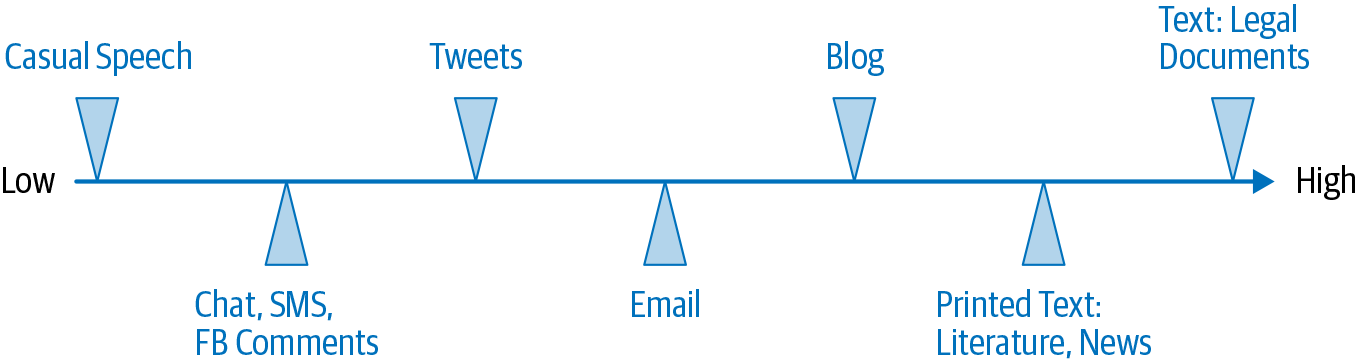
\includegraphics[width=0.65\textwidth]{capitulo3/figuras/nlp7.png}
	\caption{Espectro de formalismo en textos según sus fuentes}
	\floatfoot{Fuente: Practical natural language processing: A comprehensive guide to building real-world NLP systems \cite[p. 283]{vajjala2020practical} }
	\label{fig:nlp7}
\end{figure}

Los datos textuales provenientes de redes sociales tienden a ser considerablemente más informales en comparación con textos provenientes de blogs, libros, artículos de noticias o documentos legales.

 La Figura \ref{fig:nlp7} ilustra el espectro de formalidad en los datos de texto, ubicando diferentes fuentes de datos textuales dentro de este espectro.



Es esencial comprender la distinción entre el procesamiento de texto formal y el extremadamente informal, como el que se encuentra en las redes sociales. La labor de limpieza en este último caso debe ser más minuciosa: implica revisar exhaustivamente el texto para identificar qué aspectos se deben limpiar y qué herramientas o funciones adicionales se deben implementar para eliminar las particularidades presentes. Se requiere una cantidad significativa de tiempo y esfuerzo humano para dejar el texto en condiciones utilizables para las fases posteriores. Se hace un énfasis al esfuerzo humano debido a que el uso de herramientas existentes para el texto de redes sociales probablemente no den resultados tan satisfactorios. Estas herramientas están diseñadas para operar de manera más general y no específicamente adaptadas para manejar las características únicas que se pueden encontrar en este tipo de texto tan dinámico.